\chapter{Aufgabenstellung und Zielformulierung}

\section{Ausgangslage}

Wie bereits erwähnt, mangelt es in der Medienwelt nicht an Begeisterung für Virtual Reality. In Foren wird diskutiert, an Events wird demonstriert und täglich finden neue Infos ihren Weg in die Öffentlichkeit.

Ein wesentliches Problem ist allerdings die Benutzereingabe. Glücklicherweise gibt es bereits zu einem erschwinglichen Preis eine Möglichkeit, die eigenen zwei Hände zu verwenden und zu erkennen: die Leap Motion.

Sie ist zu einem Preis von \EUR{89.99} erhältlich \cite{leap} und ermöglicht eine rein visuelle Handerkennung ohne Handschuhe oder ähnlichen Zusatz.

\begin{figure}[h]
	\centering
	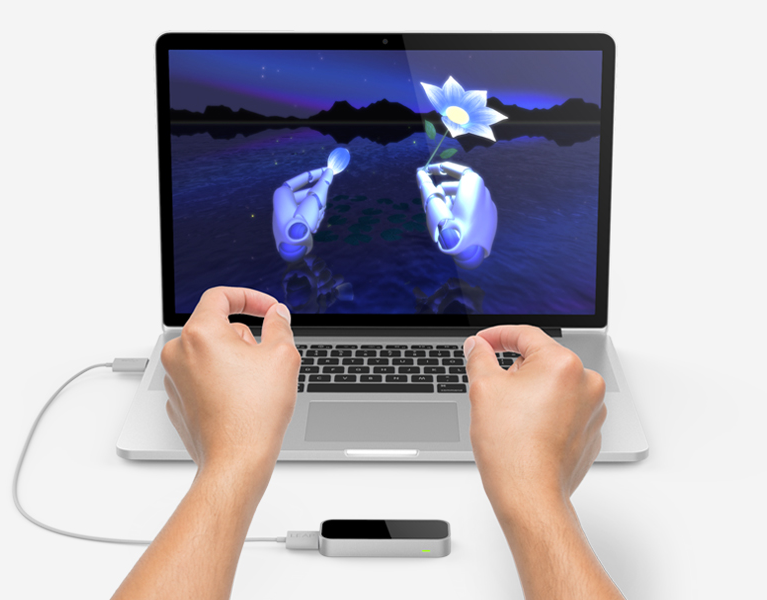
\includegraphics[width=0.5\linewidth]{bilder/leap_example}
	\caption{Die Leap Motion im Einsatz}
	\source{https://www.leapmotion.com/}
	\label{fig:leap_example}
\end{figure}

Im Vorprojekt, das ebenfalls bereits zur Sprache kam, stellte sich aus, dass jedoch Vorsicht beim Einsatz der Leap Motion geboten ist. Die Erkennung ist nicht stabil und gewisse Positionen funktionieren besser als andere. Es stellten sich also ein paar Anforderungen an eine Einbindung:

\begin{itemize}
	\item Die Applikation darf nicht auf schnelle und genaue Eingabe des Benutzers basieren
	\item Gesten müssen mit Bedacht des Sichtfeldes konzipiert werden
\end{itemize}

Besonders der erste Punkt schliesst eine Anwendung der Leap Motion in einem Spiel aus. Bei einem Spiel würden die Hände unausweichlich in den Vordergrund des Spielkonzeptes rücken und eine essenzielle Rolle übernehmen. Da allerdings die Handerkennung nicht zuverlässig ist, geschehen Fehler. Unbeabsichtigte Operationen passieren, der Spieler verliert, er ist frustriert und nach kurzer Zeit gibt er das Spiel auf.

Der gewählte Ansatz ist jedoch ein anderer: Kein Spiel soll erstellt werden, sondern eine Applikation, die durch die Hände gesteuert werden kann und dadurch einen speziellen Charme erhält. Es folgt die Zielformulierung.

\section{Ursprüngliche Zielformulierung}

Es soll eine Applikation namens ``\gls{imvr}'' (Images & Music in Virtual Reality) entwickelt werden, welche Gebrauch von der Oculus Rift macht, um die Bild- und Musiksammlung des Anwenders ansprechend darzustellen, z.B. in Form eines 3D-Karussels. Die zusätzliche ``Tiefe'', die durch den Einsatz eines stereoskopischen \gls{hmd} (Head-Mounted Display) entsteht, soll dem Anwender helfen, sich in seiner Medienbibliothek schneller zurechtzufinden.

Zusätzlich dazu soll die Leap Motion dazu verwendet werden, um vollständige Handfreiheit zu gewähren: Der Anwender soll komplett ohne Maus und Tastatur imstande sein, sich durch seine Bilder zu navigieren.

Kurz zusammengefasst muss die Applikation:

\begin{itemize}
	\item Die Bilder- und Musikbibliothek des Benutzers in stereoskopischem 3D darstellen.
	\item Diese freihändig durchsuchbar machen mit Sortier- und evtl. Gruppierfunktion.
	\item Die Bilder betrachtbar und die Musik abspielbar machen.
	\item Metainformationen darstellen (z.B. in Form von Diagrammen).
\end{itemize}

Zusätzlich zur Applikation selbst soll noch ein zusätzliches Tool entwickelt werden, welches im Voraus die Dateien auf dem Host-System indexiert und für die visuelle Applikation bereitstellt.

\section{Änderungen an der Zielformulierung}

Aufgrund der begrenzten Zeit und eines stärkeren Interesse in die Darstellung von Musik, wurde die Zielformulierung während des Projekts leicht abgeändert:

\begin{itemize}
	\item Die Bilderbibliothek fällt weg
	\item Die Sortier- und Gruppierfunktion fällt weg
	\item Es wird mehr Gewicht auf die Darstellungsweise der Musik gelegt
\end{itemize}

Dazu ist zu sagen, dass auch weiterhin stark auf die Bildervisualisierung gesetzt wird. Anstatt den Computer des Anwenders auf Bilder durchzuscannen wird diese jedoch vollständig um die lokale Musik aufgebaut. Konkret bedeutet das, dass Artwork von Alben und Fotos von Artisten dargestellt wird.

Die im zweiten Punkt erwähnte Sortier- und Gruppierfunktion könnte in einem weiteren Schritt nachgereicht werden, wurde aber im momentanen Stadium zugunsten von anderen Features vernachlässigt. Eine Gruppierung ist jedoch immer noch vorhanden in der Künstlerübersicht.

\section{Hilfsmittel \& Hardware}

Verschieden Hilfsmittel werden für die Durchführung des Projektes gebraucht. Seitens Software lauten diese:

\begin{table}[H]
	\caption{Übersicht der eingesetzten Software}
	\centering
	\label{tab:software}
	\begin{tabular}{ l l l }
		\noalign{\smallskip} \hline \hline \noalign{\smallskip}
		\textbf{Name} & \textbf{Beschreibung} \\ \midrule
		Unity3D & Spielengine und Entwicklungsumgebung \\
		Visual Studio 2012 \& 2013 & Entwicklungsumgebung von Microsoft \\
		Blender & Open-Source 3D Modelling-Tool \\
		Krita & Open-Source Grafikbearbeitungs-Tool \\
		GIMP & Open-Source Grafikbearbeitungs-Tool \\
		LaTeX & Hilfsmittel für die Erstellung wissenschaftlicher Dokumente \\
		Microsoft Visio & Tool zur Erstellung von Diagrammen \\
		\noalign{\smallskip} \hline \noalign{\smallskip}
	\end{tabular}
\end{table}

Im Hardware-Departement wurde folgendes eingesetzt:

\begin{table}[H]
	\caption{Übersicht der eingesetzten Hardware}
	\centering
	\label{tab:hardware}
	\begin{tabular}{ l l l }
		\noalign{\smallskip} \hline \hline \noalign{\smallskip}
		\textbf{Name} & \textbf{Beschreibung} \\ \midrule
		Oculus Rift & \gls{hmd} von Oculus VR \\
		Leap Motion & Hand- und Fingererkennungsgerät von Leap Motion, Inc. \\
		\noalign{\smallskip} \hline \noalign{\smallskip}
	\end{tabular}
\end{table}

Für eine genaue Erklärung der Oculus Rift und der Leap Motion sei an dieser Stelle auf das Pflichtenheft und die Vorarbeit verwiesen, welche diese im Detail einführt.
